%---------------------------------- Rotatorische Bewegung kombiniert in einem Diagramm für alle Freiheitsgrade--------------------------
\begin{center}
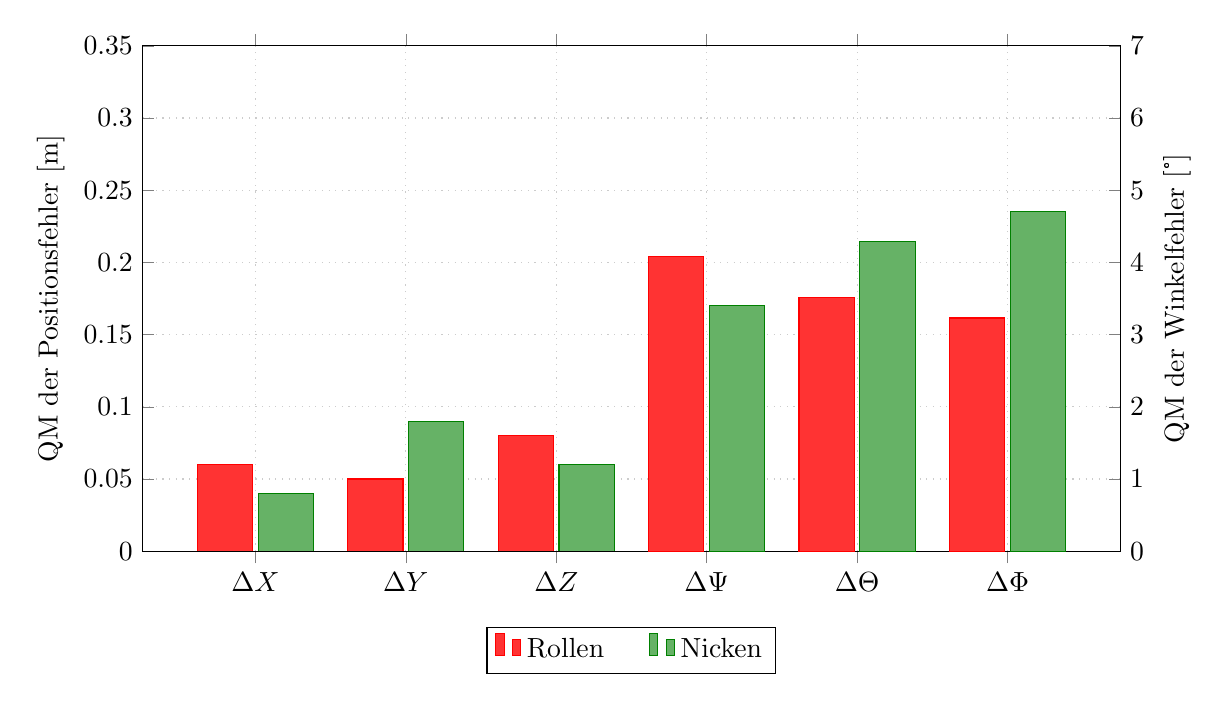
\begin{tikzpicture}
\begin{axis}[
	ybar,
	ymax=0.35,
	ymin=0,
	bar width=20pt,
	scaled y ticks = false,
	y tick label style={/pgf/number format/fixed},
%	enlarge y limits={0.4,upper},
	enlarge x limits=0.15,
	legend style={at={(0.5,-0.15)},
	legend style={/tikz/every even column/.append style={column sep=0.5cm}},
	anchor=north,legend columns=-1},
	ylabel={QM der Positionsfehler \lbrack m\rbrack},
%	symbolic x coords={\Delta,y,z},
	xtick={1,2,3,4,5,6},
	xticklabels={$\Delta X$, $\Delta Y$, $\Delta Z$, $\Delta \Psi$, $\Delta \Theta$, $\Delta \Phi$},
%	xtick=data,
%	every node near coord/.style={/pgf/number format/fixed,/pgf/number format/use comma, anchor=west},
%	nodes near coords,
%	nodes near coords align={vertical},
	width=14cm,
	height=8cm,
	grid=major,
    	grid style={dotted,lightgray!80!white},
    	scaled y ticks = false,
]
\addplot[
%	every node near coord/.append style={xshift=-0.9cm},
%	nodes near coords=\raisebox{0.7cm}{\pgfmathprintnumber\pgfplotspointmeta},
	color=Red,
	fill=Red!80!white,
	bar shift=-11pt,
] coordinates {(1,0.06) (2,0.05) (3,0.08)};
\addplot[
%	every node near coord/.append style={xshift=-0.12cm},
%	nodes near coords=\raisebox{0.7cm}{\pgfmathprintnumber\pgfplotspointmeta},
	color=Green,
	fill=Green!60!white,
	bar shift=11pt,	
] coordinates {(1,0.04) (2,0.09) (3,0.06)};
\addplot[fill opacity=0.0,draw=none,] coordinates {(4,0) (5,0) (6,0)};	%dummy
\legend{Rollen,Nicken}
\end{axis}

\begin{axis}[
%	scale only axis,
	ybar,
	ymax=7,
	ymin=0,
	bar width=20pt,
%	enlarge y limits={0.4,upper},
	enlarge x limits=0.15,
	legend style={at={(0.5,-0.15)},
	anchor=north,legend columns=-1},
	axis y line*=right,
	ylabel={QM der Winkelfehler \lbrack °\rbrack},
%	symbolic x coords={\Delta,y,z},
	xtick={1,2,3,4,5,6},
	xticklabels={},
%	xtick=data,
%	bar shift=0pt,
%	every node near coord/.style={/pgf/number format/fixed,/pgf/number format/use comma, anchor=west},
%	nodes near coords,
%	nodes near coords align={vertical},
	width=14cm,
	height=8cm,
    	scaled y ticks = false,
]
\addplot[fill opacity=0.0,draw=none,] coordinates {(1,0) (2,0) (3,0)};	%dummy
\addplot[
%	every node near coord/.append style={xshift=-0.9cm},
%	nodes near coords=\raisebox{0.7cm}{\pgfmathprintnumber\pgfplotspointmeta},
	color=Red,
	fill=Red!80!white,
	bar shift=-11pt,	
] coordinates {(4,4.08) (5,3.51) (6,3.23)};
\addplot[
%	every node near coord/.append style={xshift=-0.12cm},
%	nodes near coords=\raisebox{0.7cm}{\pgfmathprintnumber\pgfplotspointmeta},
	color=Green,
	fill=Green!60!white,
	bar shift=11pt,	
] coordinates {(4,3.40) (5,4.29) (6,4.70)};
\end{axis}
\end{tikzpicture}
\end{center}




%--------------------- Diagramm mit allen drei Rotationsbewegungen -----------------------%
%\begin{center}
%\begin{tikzpicture}
%\begin{axis}[
%	ybar,
%	ymax=0.3,
%	ymin=0,
%	bar width=10pt,
%	scaled y ticks = false,
%	y tick label style={/pgf/number format/fixed},
%%	enlarge y limits={0.4,upper},
%	enlarge x limits=0.15,
%	legend style={at={(0.5,-0.15)},
%	legend style={/tikz/every even column/.append style={column sep=0.5cm}},
%	anchor=north,legend columns=-1},
%	ylabel={Positionsfehler \lbrack m\rbrack},
%%	symbolic x coords={\Delta,y,z},
%	xtick={1,2,3,4,5,6},
%	xticklabels={$\Delta X$, $\Delta Y$, $\Delta Z$, $\Delta \Psi$, $\Delta \Theta$, $\Delta \Phi$},
%%	xtick=data,
%%	every node near coord/.style={/pgf/number format/fixed, anchor=west},
%%	nodes near coords,
%%	nodes near coords align={vertical},
%	width=14cm,
%	height=8cm,
%	grid=major,
%    	grid style={dotted,lightgray!80!white},
%    	scaled y ticks = false,
%]
%\addplot[
%%	every node near coord/.append style={xshift=-0.95cm},
%%	nodes near coords=\raisebox{0.7cm}{\pgfmathprintnumber\pgfplotspointmeta},
%	color=Red,
%	fill=Red!30!white,
%	bar shift=-12pt,
%] coordinates {(1,0.05) (2,0.11) (3,0.26)};
%\addplot[
%%	every node near coord/.append style={xshift=-0.41cm},
%%	nodes near coords=\raisebox{0.7cm}{\pgfmathprintnumber\pgfplotspointmeta},
%	color=Green,
%	fill=Green!30!white,
%	bar shift=0pt,	
%] coordinates {(1,0.11) (2,0.21) (3,0.18)};
%\addplot[
%%	every node near coord/.append style={xshift=0.12cm},
%%	nodes near coords=\raisebox{0.7cm}{\pgfmathprintnumber\pgfplotspointmeta},
%	color=Blue,
%	fill=Blue!30!white,
%	bar shift=12pt,	
%] coordinates {(1,0.21) (2,0.16) (3,0.05)};
%\addplot[fill opacity=0.0,draw=none,] coordinates {(4,0) (5,0) (6,0)};	%dummy
%\legend{Rollen,Nicken,Gieren}
%\end{axis}
%
%\begin{axis}[
%%	scale only axis,
%	ybar,
%	ymax=6,
%	ymin=0,
%	bar width=10pt,
%%	enlarge y limits={0.4,upper},
%	enlarge x limits=0.15,
%	legend style={at={(0.5,-0.15)},
%	anchor=north,legend columns=-1},
%	axis y line*=right,
%	axis x line=none,
%	ylabel={Winkelfehler \lbrack °\rbrack},
%%	symbolic x coords={\Delta,y,z},
%	xtick={1,2,3,4,5,6},
%	xticklabels={$\Delta X$, $\Delta Y$, $\Delta Z$, $\Delta \Psi$, $\Delta \Theta$, $\Delta \Phi$},
%%	xtick=data,
%%	bar shift=0pt,
%%	every node near coord/.style={/pgf/number format/fixed, anchor=west},
%%	nodes near coords,
%%	nodes near coords align={vertical},
%	width=14cm,
%	height=8cm,
%	grid=major,
%    	grid style={dotted,lightgray!80!white},
%    	scaled y ticks = false,
%]
%\addplot[fill opacity=0.0,draw=none,] coordinates {(1,0) (2,0) (3,0)};	%dummy
%\addplot[
%%	every node near coord/.append style={xshift=-0.9cm},
%%	nodes near coords=\raisebox{0.7cm}{\pgfmathprintnumber\pgfplotspointmeta},
%	color=Red,
%	fill=Red!30!white,
%	bar shift=-15pt,	
%] coordinates {(4,2) (5,2) (6,2)};
%\addplot[
%%	every node near coord/.append style={xshift=-0.12cm},
%%	nodes near coords=\raisebox{0.7cm}{\pgfmathprintnumber\pgfplotspointmeta},
%	color=Green,
%	fill=Green!30!white,
%	bar shift=0pt,	
%] coordinates {(4,3) (5,3) (6,3)};
%\addplot[
%%	every node near coord/.append style={xshift=-0.12cm},
%%	nodes near coords=\raisebox{0.7cm}{\pgfmathprintnumber\pgfplotspointmeta},
%	color=Blue,
%	fill=Blue!30!white,
%	bar shift=15pt,	
%] coordinates {(4,4) (5,4) (6,4)};
%\end{axis}
%\end{tikzpicture}
%\end{center}
%--------------------- Diagramm mit allen drei Rotationsbewegungen -----------------------%




